\documentclass{article}

\usepackage{fancyhdr}
\usepackage{extramarks}
\usepackage{amsmath}
\usepackage{amsthm}
\usepackage{amsfonts}
\usepackage{tikz}
\usepackage[plain]{algorithm}
\usepackage{algpseudocode}
\usepackage{graphicx}
\usetikzlibrary{automata,positioning}
\usepackage{csvsimple}
\usepackage{hyperref}
\usepackage{natbib}
%
% Basic Document Settings
%

\topmargin=-0.45in
\evensidemargin=0in
\oddsidemargin=0in
\textwidth=6.5in
\textheight=9.0in
\headsep=0.25in

\linespread{1.1}

\pagestyle{fancy}
\lhead{\hmwkAuthorName}
\chead{\hmwkClass \hmwkTitle}
%\rhead{\firstxmark}
\rhead{\authorID}
%\lfoot{\lastxmark}
\cfoot{\thepage}

\renewcommand\headrulewidth{0.4pt}
\renewcommand\footrulewidth{0.4pt}

\setlength\parindent{0pt}

%
% Create Problem Sections
%

\newcommand{\enterProblemHeader}[1]{
    \nobreak\extramarks{}{Problem \arabic{#1} continued on next page\ldots}\nobreak{}
    \nobreak\extramarks{Problem \arabic{#1} (continued)}{Problem \arabic{#1} continued on next page\ldots}\nobreak{}
}

\newcommand{\exitProblemHeader}[1]{
    \nobreak\extramarks{Problem \arabic{#1} (continued)}{Problem \arabic{#1} continued on next page\ldots}\nobreak{}
    \stepcounter{#1}
    \nobreak\extramarks{Problem \arabic{#1}}{}\nobreak{}
}

\setcounter{secnumdepth}{0}
\newcounter{partCounter}
\newcounter{homeworkProblemCounter}
\setcounter{homeworkProblemCounter}{1}
\nobreak\extramarks{Problem \arabic{homeworkProblemCounter}}{}\nobreak{}

%
% Homework Problem Environment
%
% This environment takes an optional argument. When given, it will adjust the
% problem counter. This is useful for when the problems given for your
% assignment aren't sequential. See the last 3 problems of this template for an
% example.
%
\newenvironment{homeworkProblem}[1][-1]{
    \ifnum#1>0
        \setcounter{homeworkProblemCounter}{#1}
    \fi
    \section{Problem \arabic{homeworkProblemCounter}}
    \setcounter{partCounter}{1}
    \enterProblemHeader{homeworkProblemCounter}
}{
    \exitProblemHeader{homeworkProblemCounter}
}

%
% Homework Details
%   - Title
%   - Due date
%   - Class
%   - Section/Time
%   - Instructor
%   - Author
%

\newcommand{\hmwkTitle}{Assignment\ \#2}
\newcommand{\hmwkDueDate}{\date{\today}}
\newcommand{\hmwkClass}{Computer Vision}
\newcommand{\authorID}{pm2758}
\newcommand{\hmwkClassTime}{Section A}
\newcommand{\hmwkClassInstructor}{Prof Rob Fergus}
\newcommand{\hmwkAuthorName}{\textbf{Pramit Mallick}}

%
% Title Page
%

\title{
    \vspace{2in}
    \textmd{\textbf{\hmwkClass:\ \hmwkTitle}}\\
    \normalsize\vspace{0.1in}\small{\hmwkDueDate}
%    \vspace{0.1in}\large{\textit{\hmwkClassInstructor\ \hmwkClassTime}}
    \vspace{3in}
}

\author{\hmwkAuthorName \\ \authorID}
\date{}

\renewcommand{\part}[1]{\textbf{\large Part \Alph{partCounter}}\stepcounter{partCounter}\\}

%
% Various Helper Commands
%

% Useful for algorithms
\newcommand{\alg}[1]{\textsc{\bfseries \footnotesize #1}}

% For derivatives
\newcommand{\deriv}[1]{\frac{\mathrm{d}}{\mathrm{d}x} (#1)}

% For partial derivatives
\newcommand{\pderiv}[2]{\frac{\partial}{\partial #1} (#2)}

% Integral dx
\newcommand{\dx}{\mathrm{d}x}

% Alias for the Solution section header
\newcommand{\solution}{\textbf{\large Solution}}

% Probability commands: Expectation, Variance, Covariance, Bias
\newcommand{\E}{\mathrm{E}}
\newcommand{\Var}{\mathrm{Var}}
\newcommand{\Cov}{\mathrm{Cov}}
\newcommand{\Bias}{\mathrm{Bias}}

\begin{document}

\maketitle

\pagebreak
Taking a closer look at the dataset, we realized that any normal network would require a lot of data augmentation to help train instances where an image or the region of interest in the image is rotated and scaled and cropped. Augmenting data and adding more CNN layers and fully connected layers into the given base model could've solved the problem by brute force if trained for enough epochs, but it would be prone to overfitting. After some research, we found the Spatial Transformer Network (STN) by \cite{jaderberg2015spatial} to be an interesting solution to the problem. STNs allow a neural network to learn how to perform spatial transformations on the input image in order to enhance the geometric invariance of the model. 
We trained a simple STN and achieved the following results -
\begin{center}
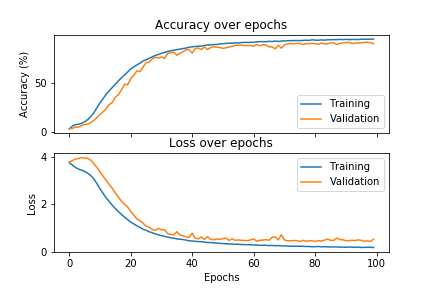
\includegraphics[width=0.5\textwidth]{model_stn.png}
\end{center}
But it only achieved 91.44\% accuracy on the validation set and 0.94726 score on the test set.\\
Closer inspection showed us that the model was oscillating in its error rate after a certain epoch, suggesting that the step size must be reduced. Thus to ensure convergence, I reduced the learning rate by half when the validation accuracy reached 80\%, then again at 85\% and finally at 90\%. I also added another convolution layer (increased the number of filters at each stage as well), introduced batch normalization and added another fully connected layer at the end. This lead to the model performing 95.47\% on the validation set and 0.97149 score on the test set. The convergence results are -
\begin{center}
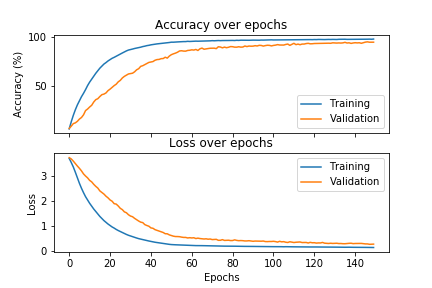
\includegraphics[width=0.5\textwidth]{model_stn_lr2_conv.png}
\end{center}
The relevant model is included in the zipped attachment with the name \textbf{\texttt{model\_stn\_lr2\_conv.pth}}.


\bibliographystyle{plainnat}
\bibliography{ref}

\end{document}
